\documentclass{article}

\usepackage{tikz}

\begin{document}
    \tikz \draw[line width=.2cm] (0,0) - - (1,1); 
    \tikz \draw[line width=.2cm] (0,0) - - (1,1);
    \tikz \draw (0,0) - - (2,1);

    \tikz \draw (0, 0) -- (2, 1);
    \tikz \draw (0, 0) |- (2, 1);
    \tikz \draw(0, 2) .. controls(3, 0) .. (2, 2);
    \tikz \draw(0, 2) .. controls(3, 0) and (-1, 0) .. (2, 2);
    \tikz \fill(0, 2) .. controls(3, 0) and (-1, 0) .. (2, 2);
    \tikz \filldraw (0, 2) .. controls(3, 0) and (-1, 0) .. (2, 2);

    \tikz \draw (0, 0) rectangle(3, 2);

    \tikz \draw(1, 1) circle(1);

    \tikzset{dfr/.pic={         \filldraw[blue] (-2pt, 0) rectangle(0, 5pt);
        \filldraw[fill=white] (0, 0) rectangle(2pt, 5pt);
        \filldraw[fill=red] (2pt, 0) rectangle (4pt, 5pt);}}

    \tikz \pic at (1, 1) [pic type = dfr];
    \tikz \pic (1, 1) {dfr};
    \tikz \pic[scale=3, rotate=45, red] (1, 1) {dfr};

    \tikz \draw (0, 0) to [out=10, in=170] pic [near start] {dfr} pic {dfr} pic [sloped, near end] {dfr} (10, 0);

    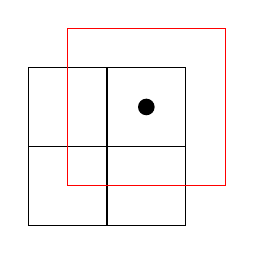
\begin{tikzpicture}
        
        \draw (0, 0) grid (2, 2);
        %坐标
        \coordinate (center) at (1.5, 1.5);
        \coordinate (A) at (.5, .5);
        \coordinate (B) at (2.5, 2.5);
        \fill (center) circle (3pt);
        \draw[red] (A) rectangle (B);

    \end{tikzpicture}

    \tikz \fill [fill=blue!50, draw=blue, very thick](0, 0) node [behind path, fill=red!50] {XXXXX} -- (1.5, 0) -- (1.5, 1) -- (0, 1);

    % node
    % \usetikzlibrary{shapes.geometric}
    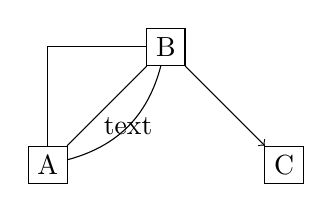
\begin{tikzpicture}
        \node[draw] (A) at (0, 0) {A};
        \node [draw] (B) at (1.5, 1.5) {B};
        \node [draw] (C) at (3, 0) {C};
        \draw (A) -- (B);
        \draw (A) |- (B);
        \draw (A) to [bend right] node [bend right] {text} (B);
        \draw (B) edge[->]  (C);
    \end{tikzpicture}

    \tikz \fill(0, 0) circle (2pt) node[above] {text};

    %scope


    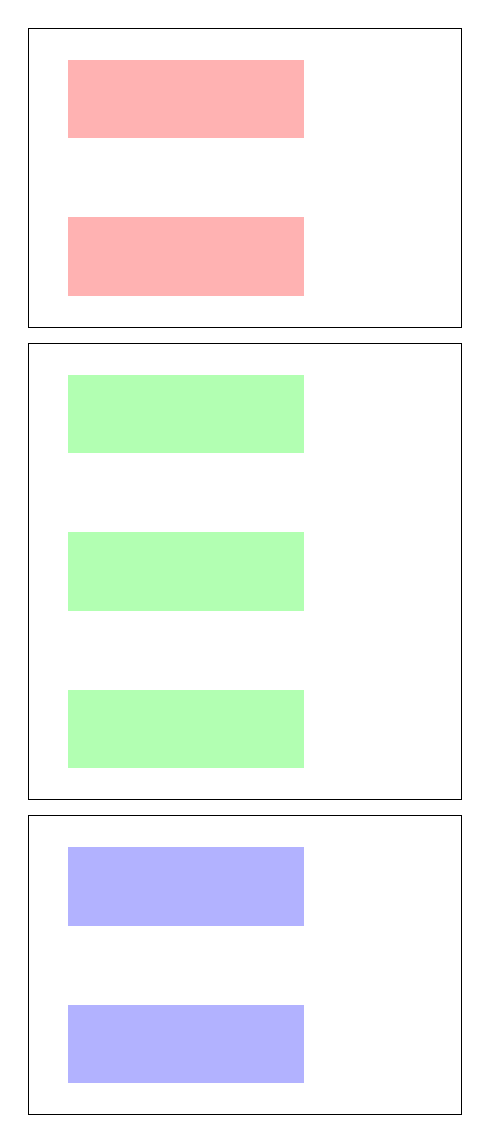
\begin{tikzpicture}
        \begin{scope}
            \fill[red!30!white]   (0, 11) rectangle (3, 12);
            \fill[red!30!white]   (0, 9) rectangle (3, 10);
            \fill[green!30!white] (0, 7) rectangle (3, 8);
            \fill[green!30!white] (0, 5) rectangle (3, 6);
            \fill[green!30!white] (0, 3) rectangle (3, 4);
            \fill[blue!30!white]  (0, 1) rectangle (3, 2);
            \fill[blue!30!white]  (0, -1) rectangle (3, 0);

            \draw (-.5, 8.6) -- (5, 8.6) -- (5, 12.4) -- (-.5, 12.4) -- cycle;
            \draw (-.5, 2.6) -- (5, 2.6) -- (5, 8.4) -- (-.5, 8.4) -- cycle;
            \draw (-.5, -1.4) -- (5, -1.4) -- (5, 2.4) -- (-.5, 2.4) -- cycle;

        \end{scope}
        
    \end{tikzpicture}


\end{document}